\chapter{Results}
\label{results}

In this chapter we present the results of our simulation. In the first section we will present the default and individualized lifecycle investment strategies, the former being provided by real retirement funds and the latter being solved by Merton and Munk. We will plug in the heterogeneous parameters, described in detail in the previous chapter. In the next section, we will calculate the resulting financial capital flows and compare their welfare effects using their expected utilities, as mentioned in Chapter 3. 

\section{Investment strategies}
\subsection{Default lifecyccles}
As was discussed in the previous chapter, our individual decides between investing in risky (stocks) or risk-free (bonds) assets. The default allocations for share of risky asset are given by:

\begin{itemize}
	\item $100-t$, for all $t$
	\item $\begin{cases} 100\%, & t<40\\(200-2.5t)\%, & t\in[40,57]\end{cases}$
	\item $63\%$, for all $t$
	\item $30\%$, for all $t$
\end{itemize}

where the latter two are Markowitz's solution and Anadolu Hayat's moderate investment option respectively. Since we are only interested in age span between 28 and 57, Figure 5.1 shows the risky asset share $\pi_t$ only for that interval. 

\begin{figure}[h]
	\centering
	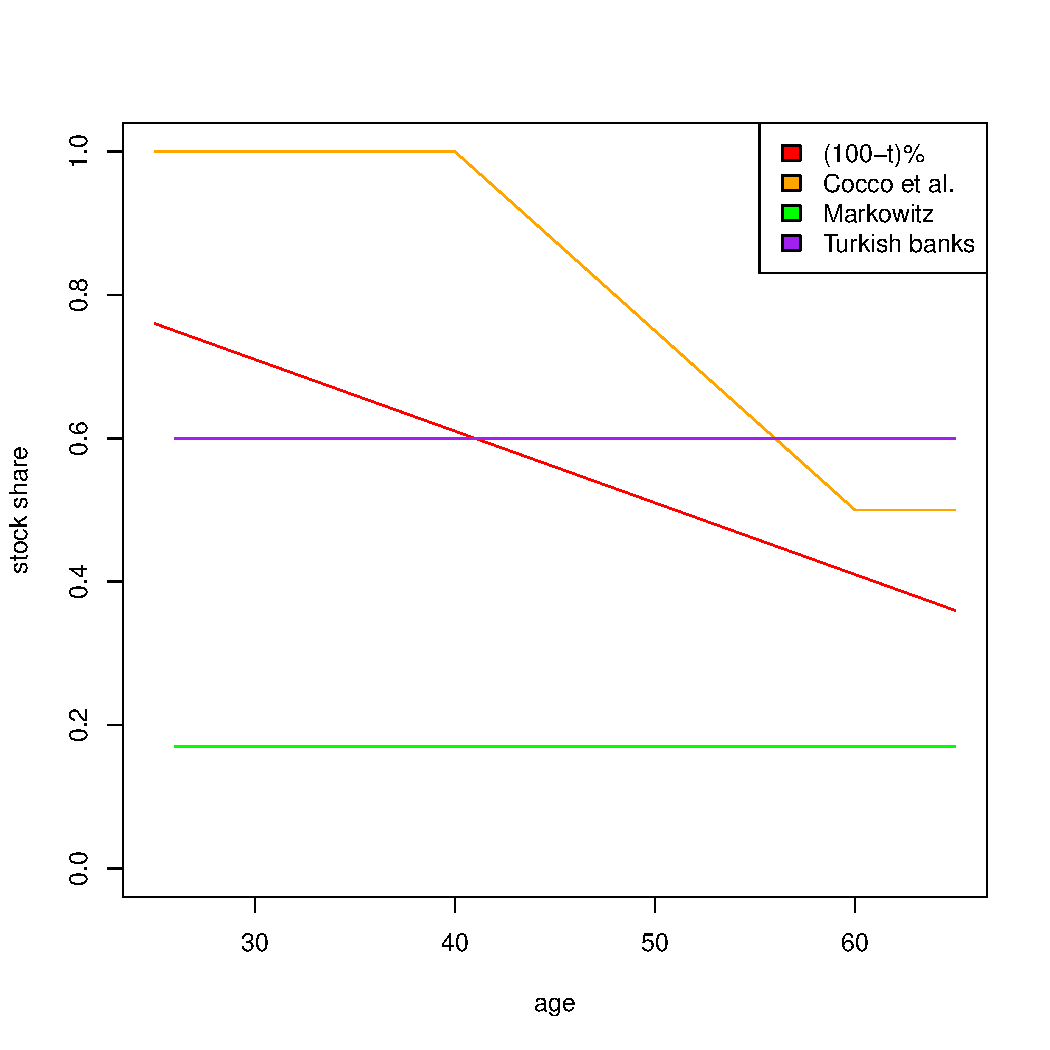
\includegraphics[scale=0.6]{figs/defaults.pdf}
	\caption{Default portfolio allocations of stock investments}
\end{figure}


\subsection{Individualized lifecycles}

To derive individualized lifecycle strategies, we used Merton's (1971) and Munk's (2016) optimal portfolio allocation formulas mentioned in chapters 2 and 3. Since these formulas depended on intratemporal amounts of capital, we have constructed three human capital series corresponding to flat, moderate and steep wage growth curves mentioned in the previous chapter. Figure 5.2 illustrates the risky asset shares given by Merton and Munk without housing for various levels of labor income growth and risk aversion. The figure shows that the steeper the wage growth curves get or the lower their risk aversion is, the more aggressive investors are. However, as a whole, they follow the similar pattern. The figure also shows that for small correlations between labor income and stock prices, Munk's solution converges to Merton's solution, as was shown in Chapter 3.

\begin{figure}
	\centering
    \begin{subfigure}{0.45\textwidth}
		\centering
		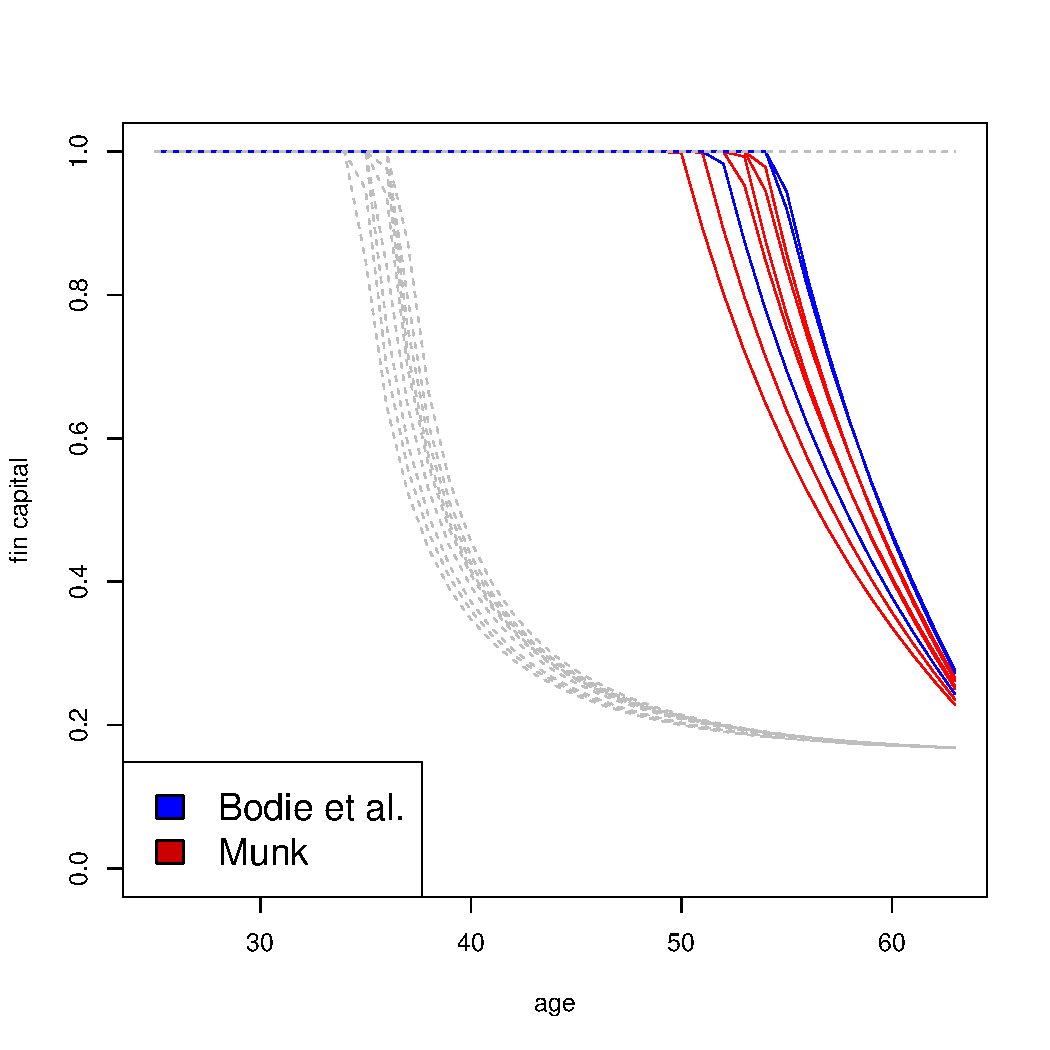
\includegraphics[scale=0.4]{figs/individuals15.pdf}
		\caption{$\gamma = 1.5$}
	\end{subfigure}
	\hfill
    \begin{subfigure}{0.45\textwidth}
		\centering
		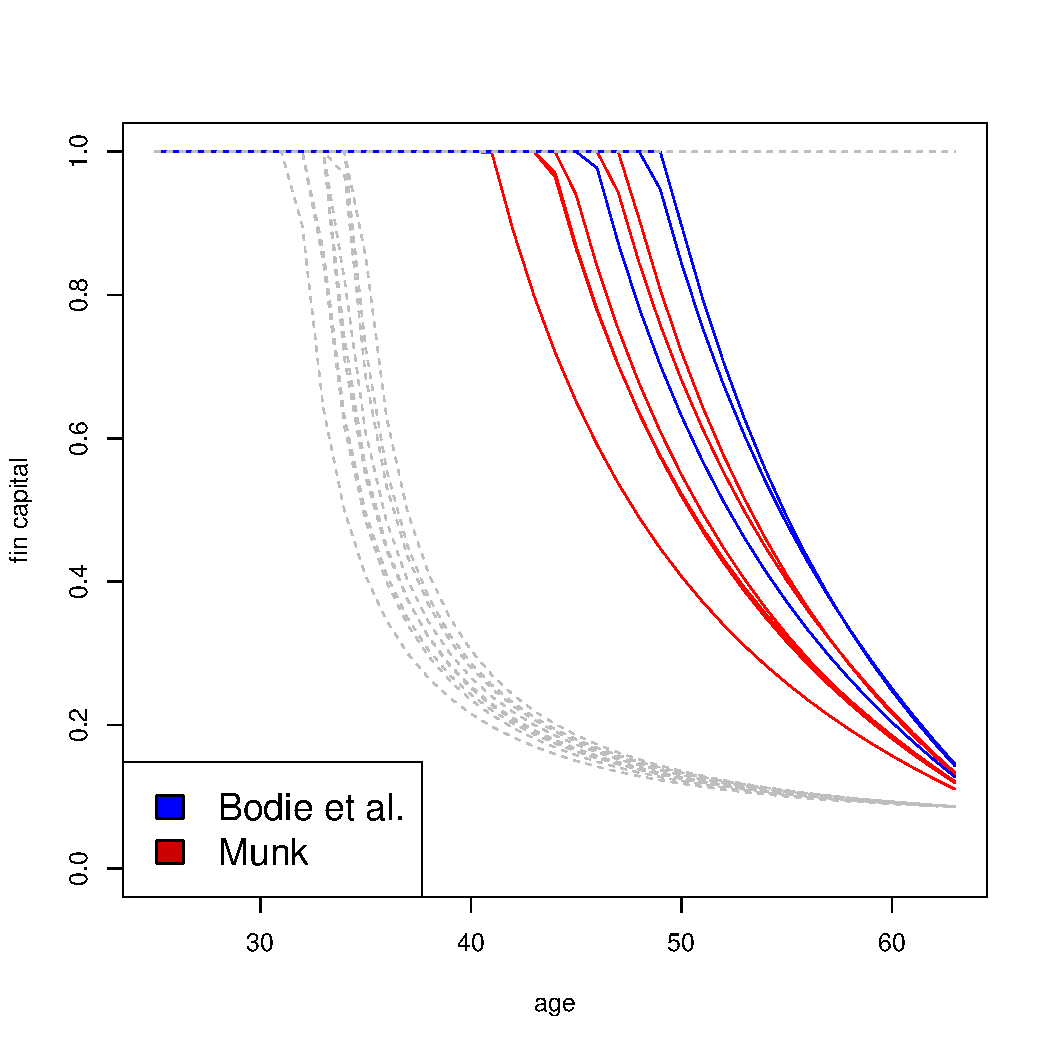
\includegraphics[scale=0.4]{figs/individuals3.pdf}
		\caption{$\gamma = 3$}
	\end{subfigure}
	\hfill
    \begin{subfigure}{0.45\textwidth}
		\centering
		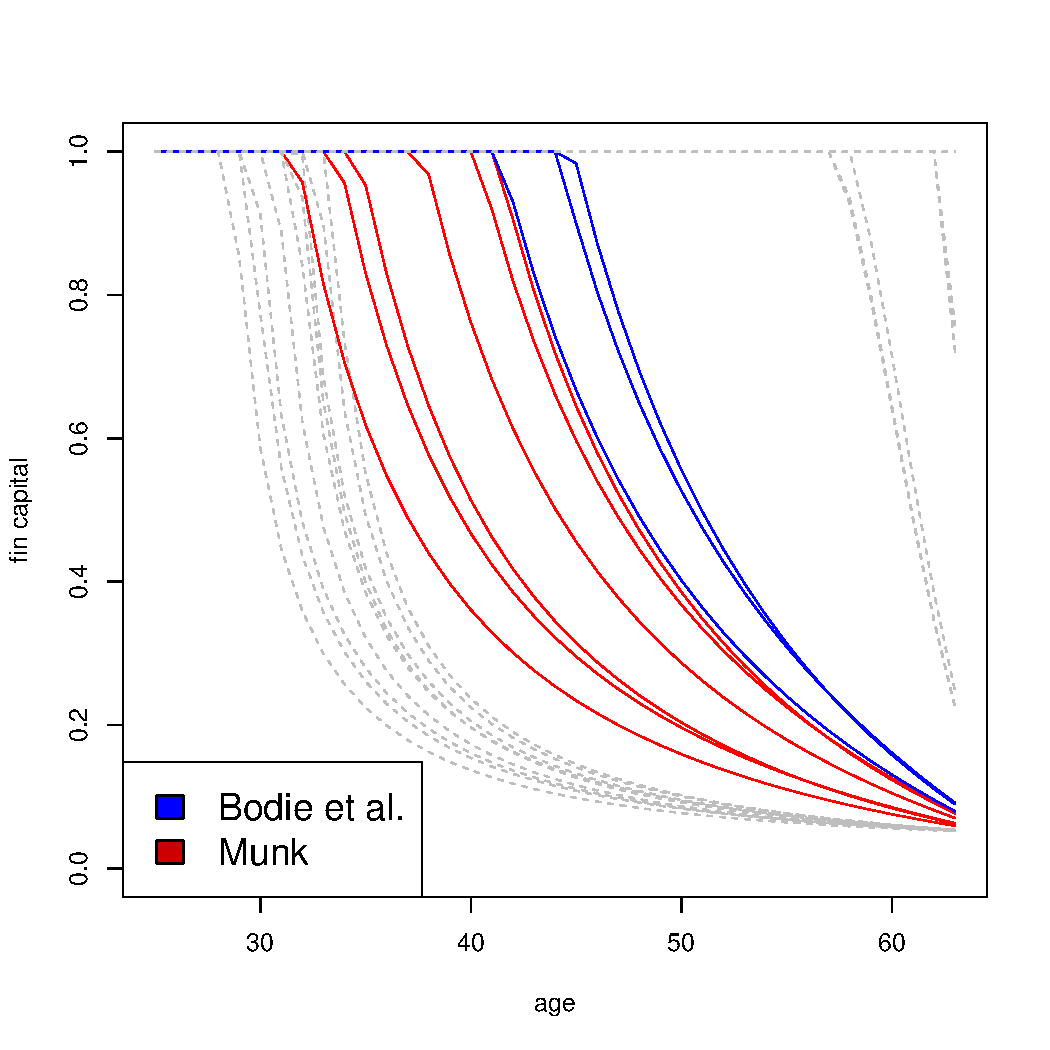
\includegraphics[scale=0.4]{figs/individuals5.pdf}
		\caption{$\gamma = 5$}
	\end{subfigure}
	\hfill
    \begin{subfigure}{0.45\textwidth}
		\centering
		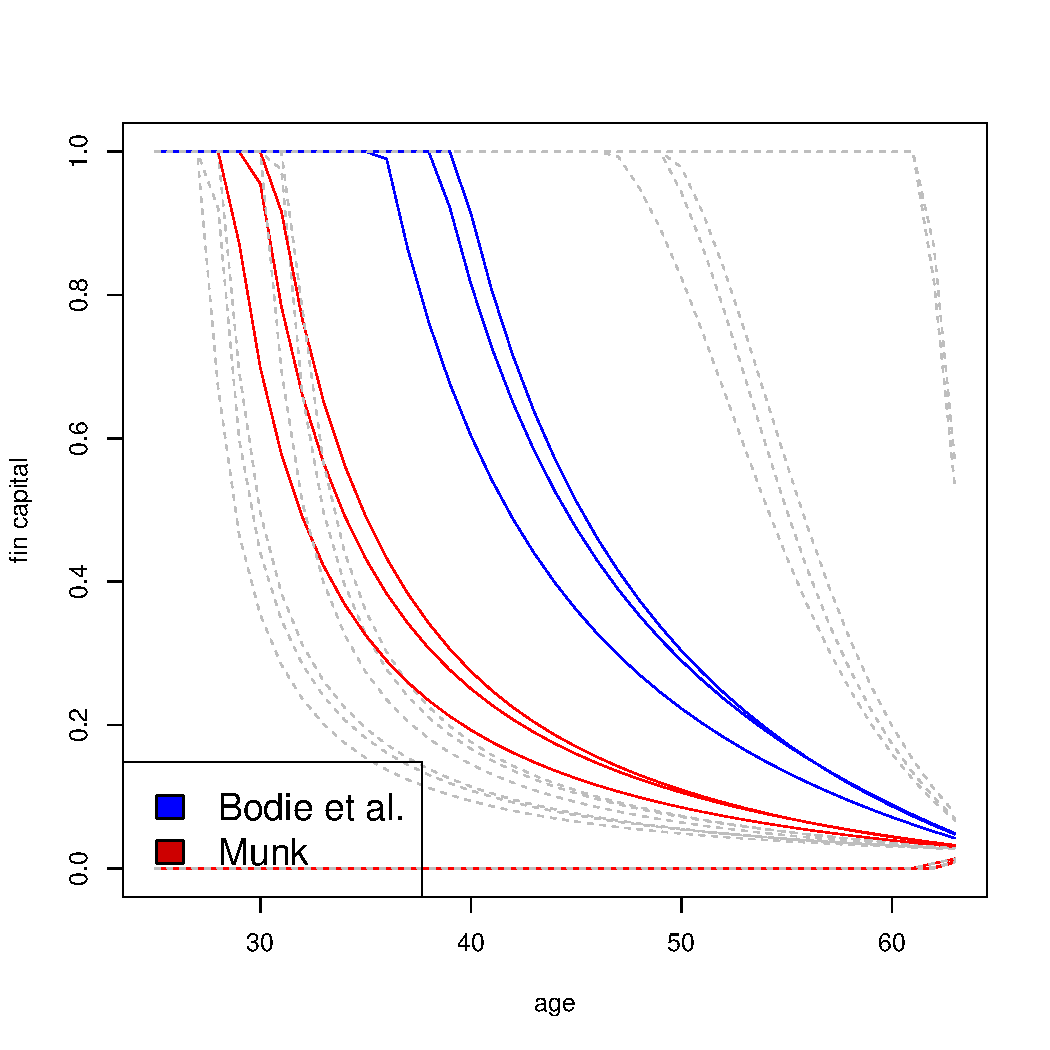
\includegraphics[scale=0.4]{figs/individuals10.pdf}
		\caption{$\gamma = 10$}
	\end{subfigure}
	\caption{Merton and Munk's solution without housing for different wage growth and risk aversion levels}
\end{figure}

\paragraph{}Figure 5.3 illustrates the stock and housing asset shares determined by Munk with housing for flat, moderate and steep labor income curves and low, moderate and high stock-labor income correlations for different levels of risk aversion, to capture heterogeneity, as mentioned in the previous chapter. The figure confirms that steeper labor income curves result in larger share of stocks in portfolio and less of bonds. Around age of 45, the sum of optimal stock and housing investments falls below $1$ and optimal bond investment becomes positive. Also, the higher the risk aversion, the less the individuals want to invest in both housing and stocks --- for $\gamma=10$, the optimal Munk solutions are negative or add up to less than $1$, meaning that they should sell all stocks and housing to invest in risk-free long term bonds. In our analysis we do not allow for negative investing, since this is not a primary focus of our thesis.  



\paragraph{}Full tables with actual solutions are available in Tables E.1 and E.2 of Appendix E for models without housing and in Table E.3 for a model with housing. 


\section{Welfare comparison}

In order to compare welfare we use CRRA expected utility function, mentioned in Chapter 3. The probabilities of survival are taken from TUIK as mentioned in the previous chapter. The consumption is calculated in numbers of consumption baskets which cost exactly $1$ CPI --- consumer price index at that period, which is increasing with inflation rate annually, and is equal to $100$ at retirement age $57$. The wealth for which consumption baskets are purchased is a total accumulated wealth, including stock returns, bond returns and housing returns, annuitized according to the formula described in Chapter 3. Discount rate is $0.89$, as mentioned in the previous chapter. We compare expected utilities for different levels of risk aversion.

\begin{figure}[H]
	\centering
    \begin{subfigure}{0.45\textwidth}
		\centering
		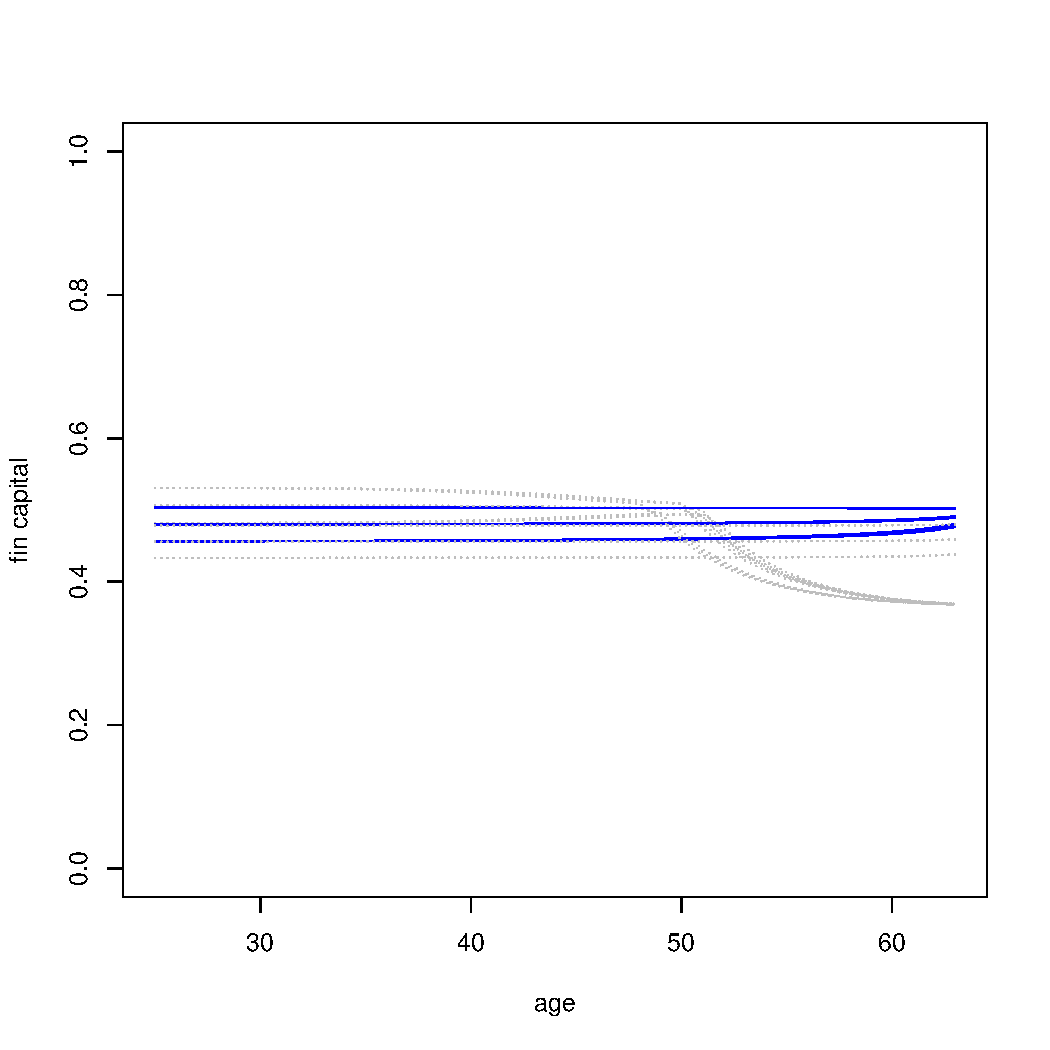
\includegraphics[scale=0.4]{figs/smunkhouse15.pdf}
		\caption{Stocks for $\gamma = 1.5$}
	\end{subfigure}
	\hfill
    \begin{subfigure}{0.45\textwidth}
		\centering
		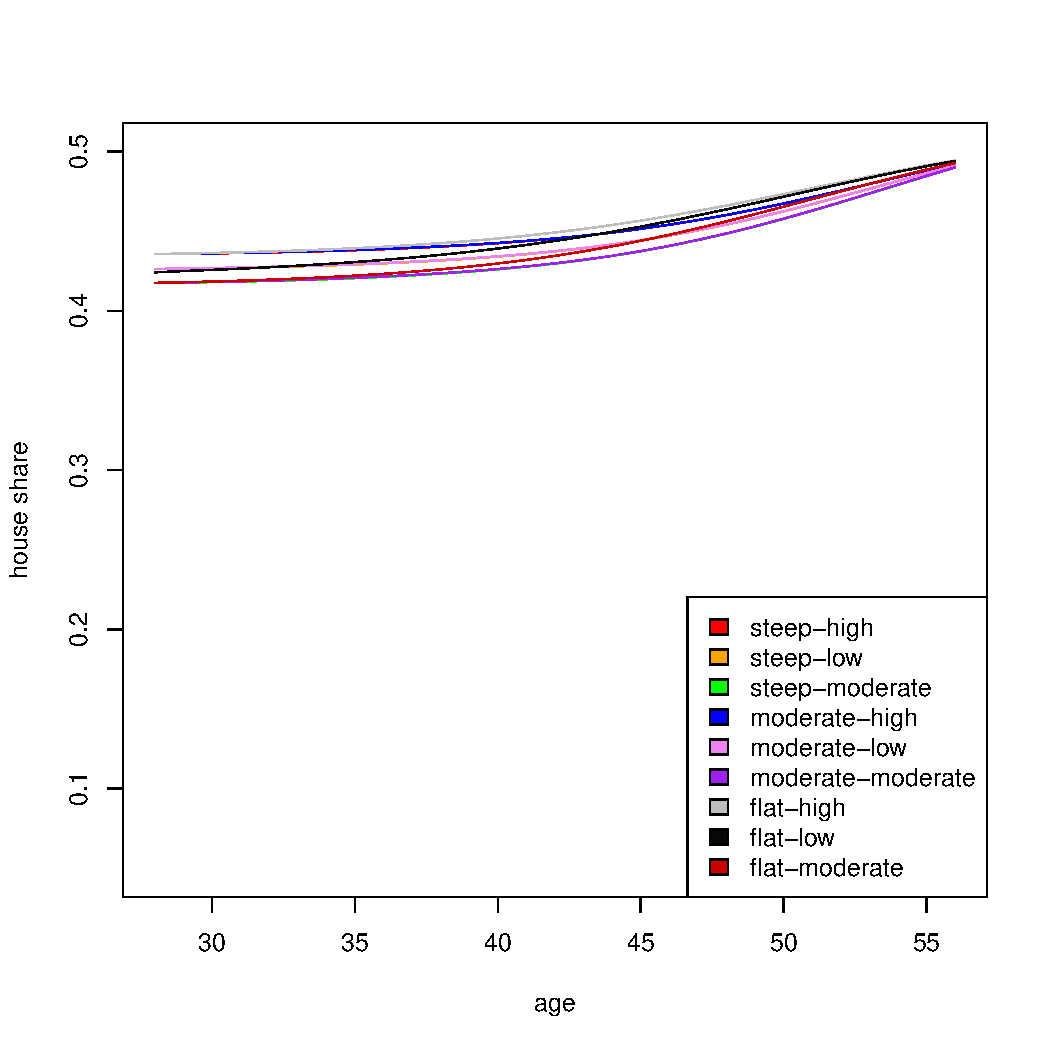
\includegraphics[scale=0.4]{figs/hmunkhouse15.pdf}
		\caption{Housing for $\gamma = 1.5$}
	\end{subfigure}
	\hfill
    \begin{subfigure}{0.45\textwidth}
		\centering
		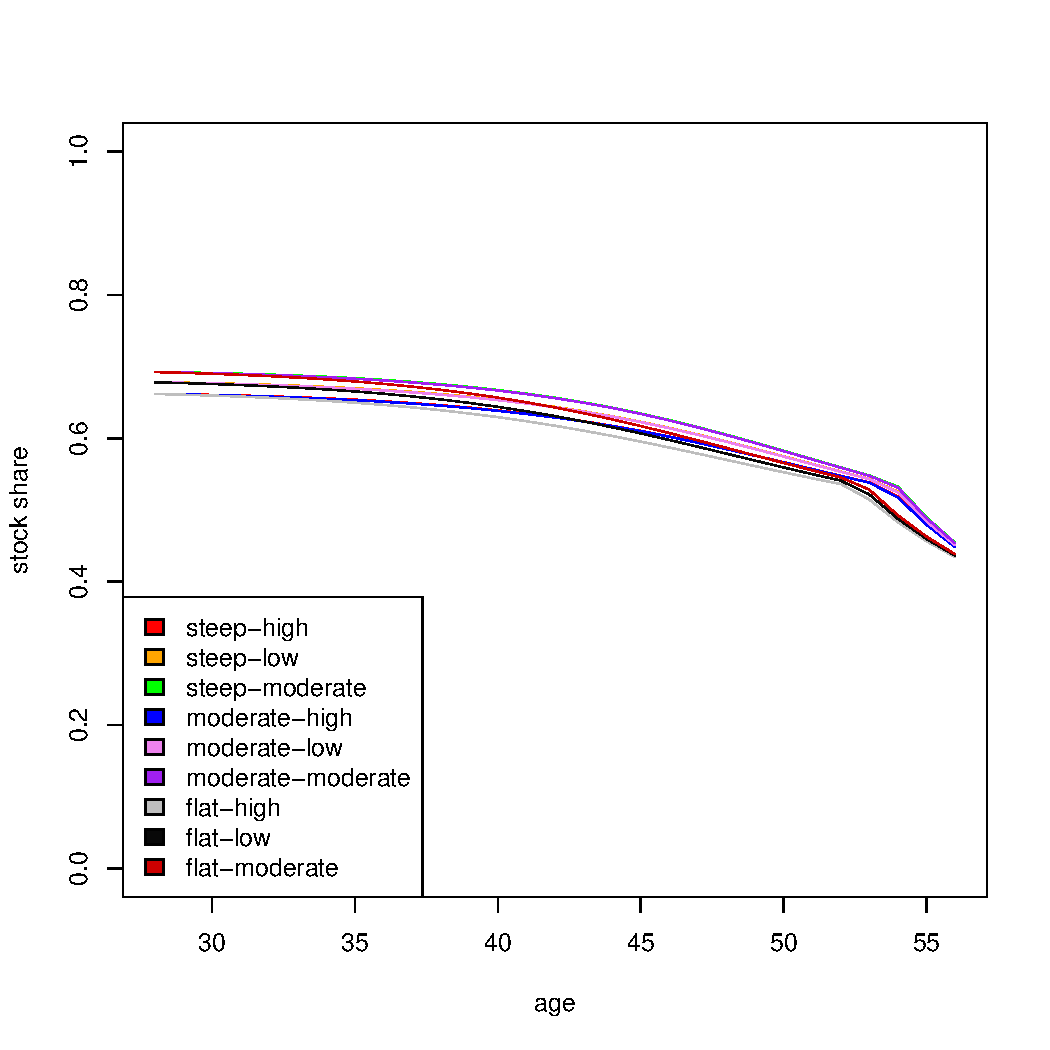
\includegraphics[scale=0.4]{figs/smunkhouse3.pdf}
		\caption{Stocks for $\gamma = 3$}
	\end{subfigure}
	\hfill
    \begin{subfigure}{0.45\textwidth}
		\centering
		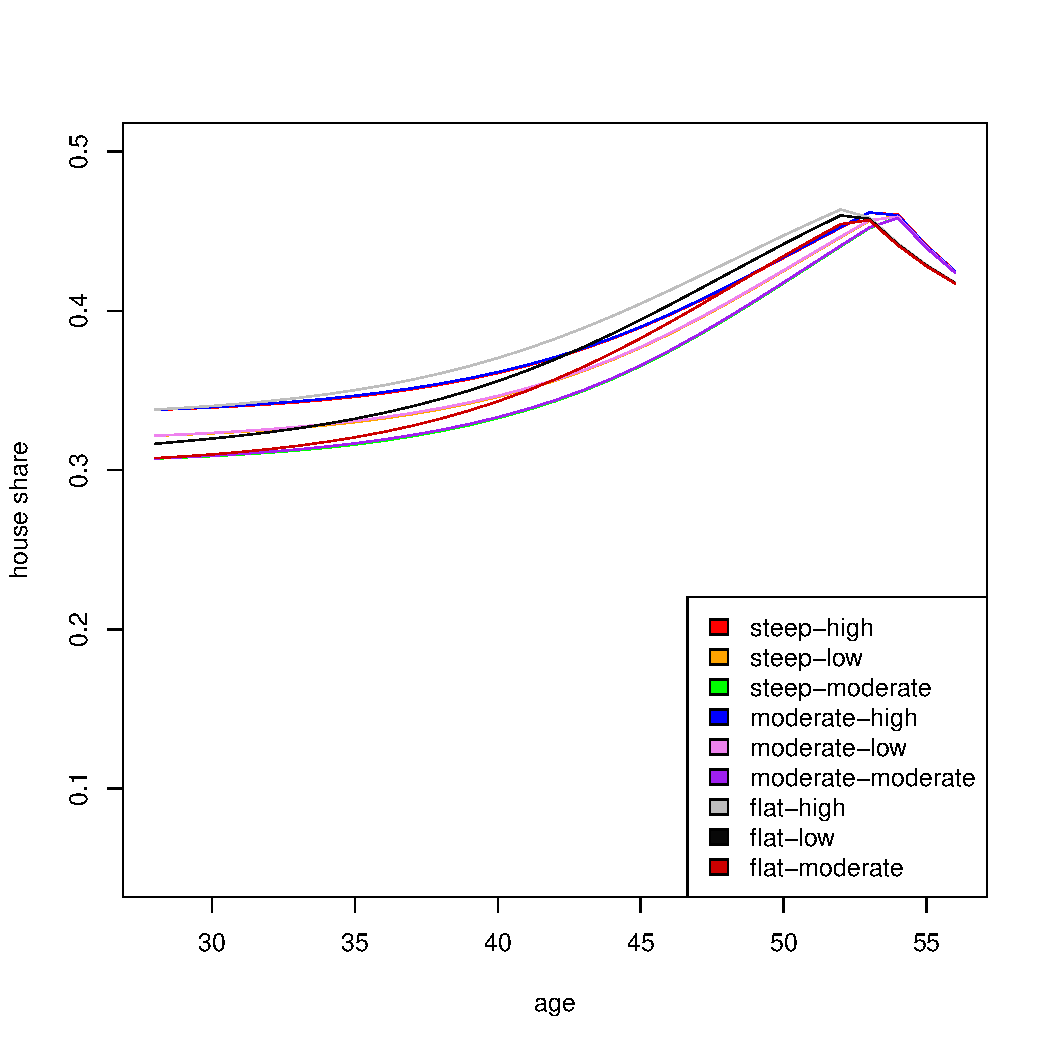
\includegraphics[scale=0.4]{figs/hmunkhouse3.pdf}
		\caption{Housing for $\gamma = 3$}
	\end{subfigure}
	\hfill
    \begin{subfigure}{0.45\textwidth}
		\centering
		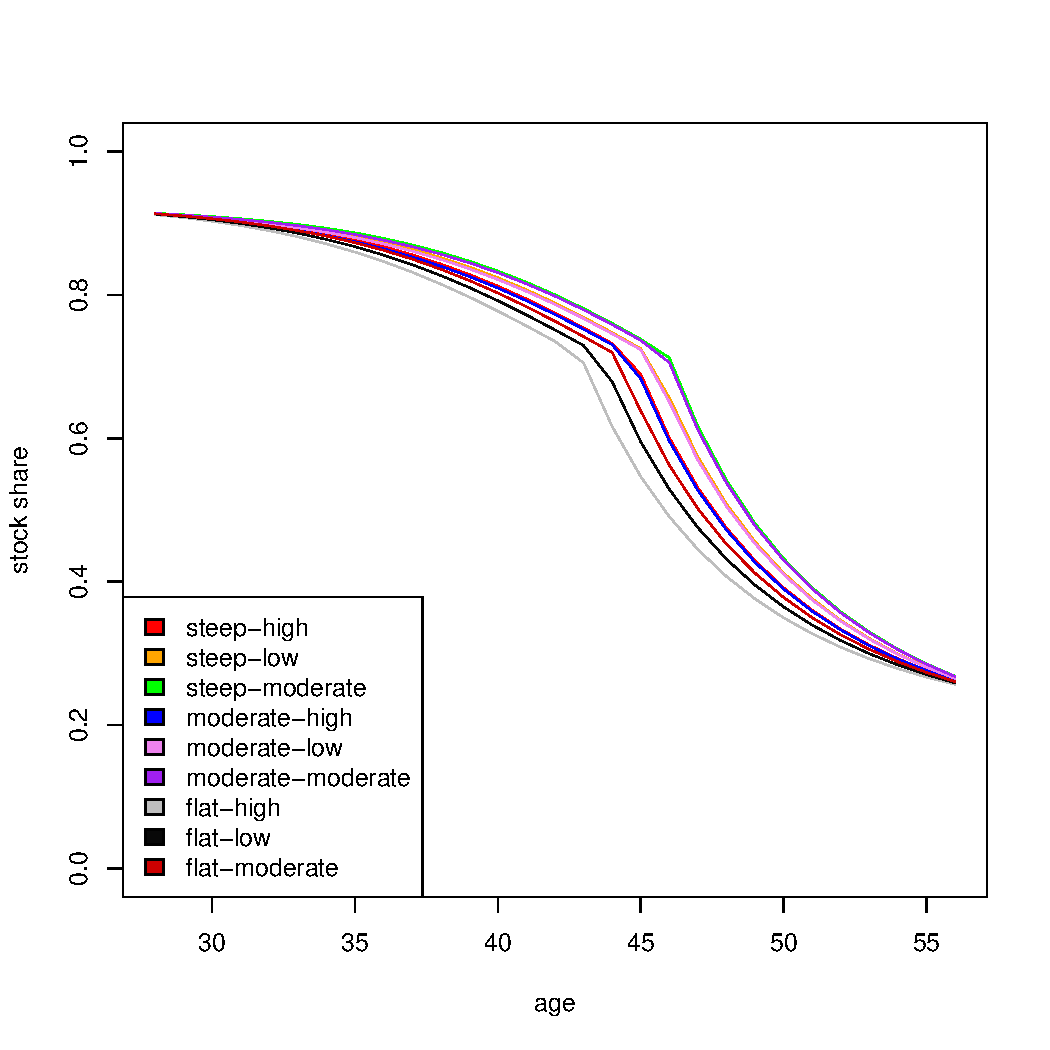
\includegraphics[scale=0.4]{figs/smunkhouse5.pdf}
		\caption{Stocks for $\gamma = 5$}
	\end{subfigure}
	\hfill
    \begin{subfigure}{0.45\textwidth}
		\centering
		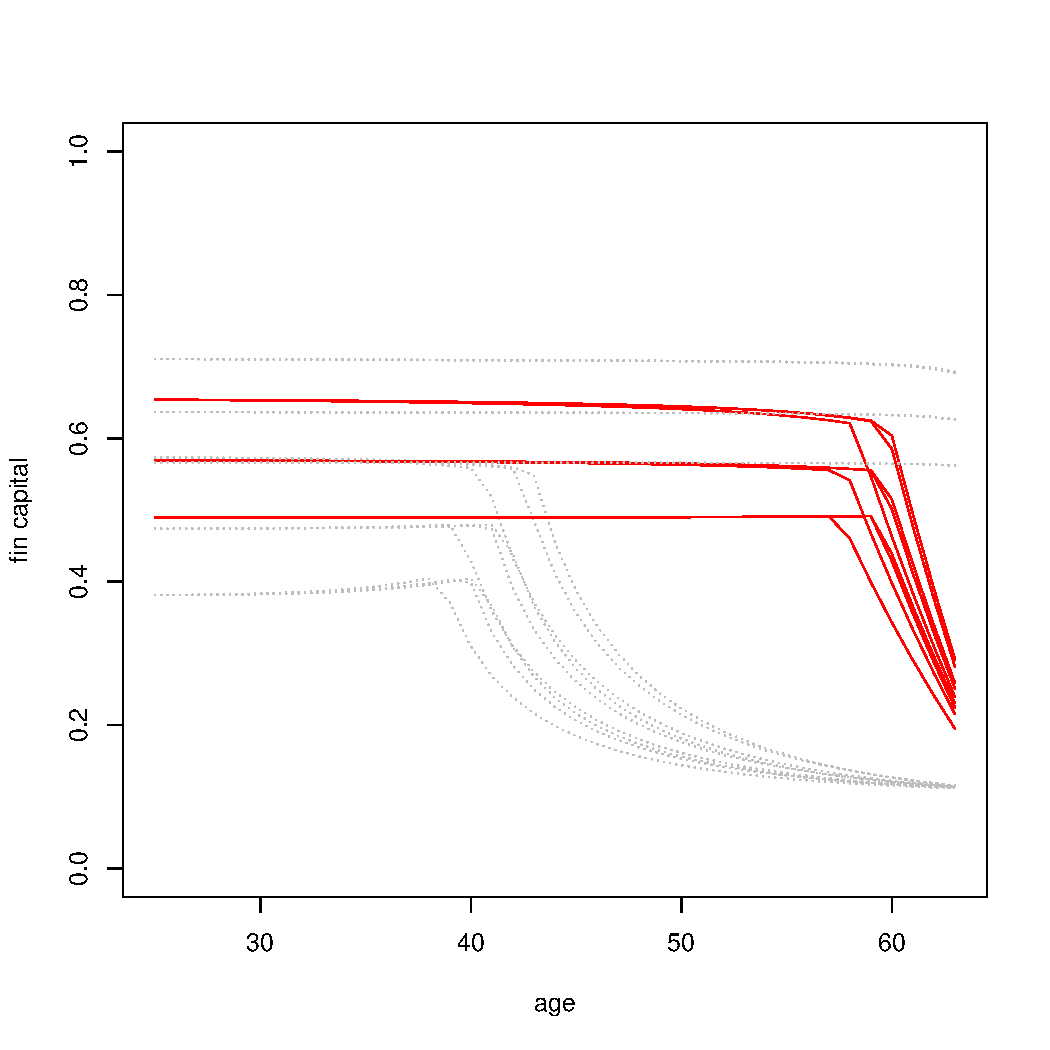
\includegraphics[scale=0.4]{figs/hmunkhouse5.pdf}
		\caption{Housing for $\gamma = 5$}
	\end{subfigure}
\end{figure}
\begin{figure}[H]\ContinuedFloat
    \begin{subfigure}{0.45\textwidth}
		\centering
		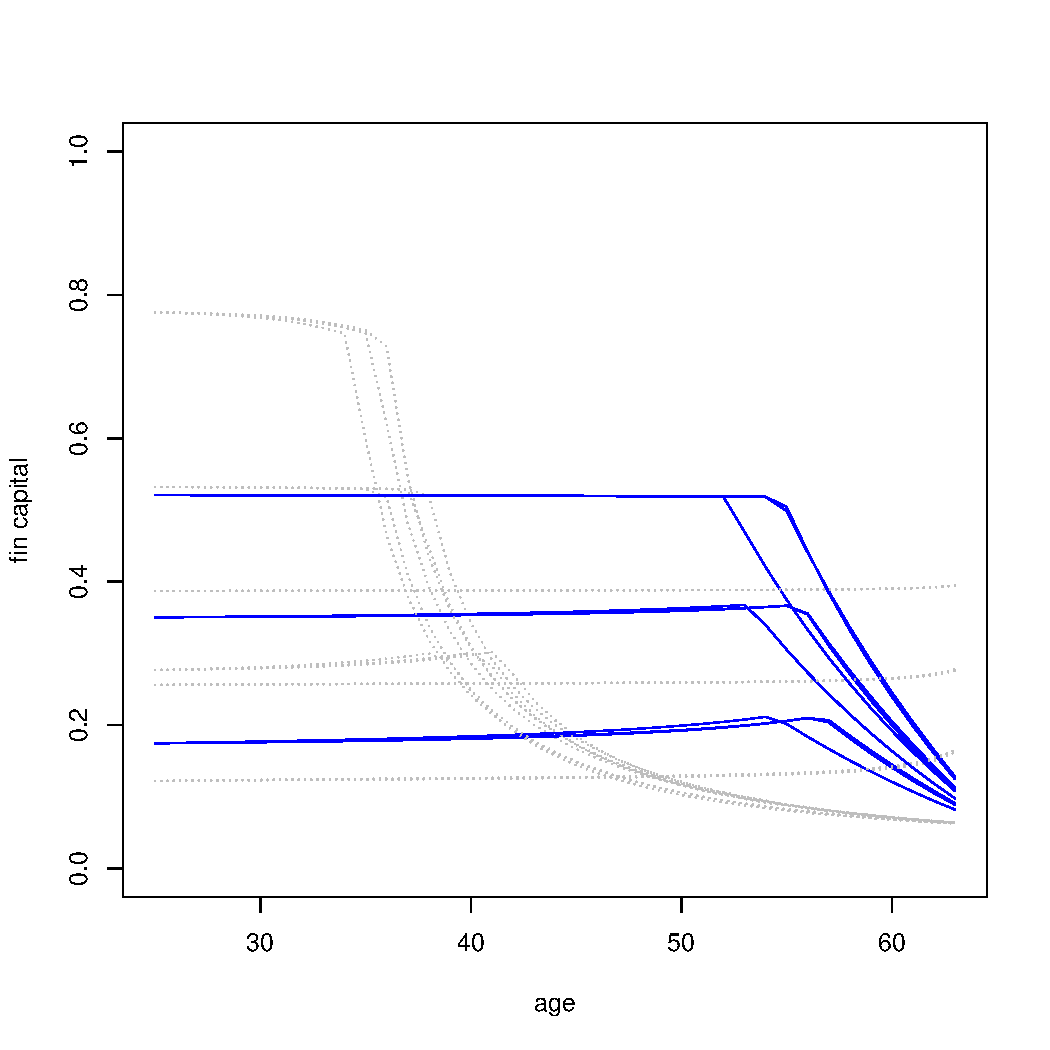
\includegraphics[scale=0.4]{figs/smunkhouse10.pdf}
		\caption{Stocks for $\gamma = 10$}
	\end{subfigure}
	\hfill
    \begin{subfigure}{0.45\textwidth}
		\centering
		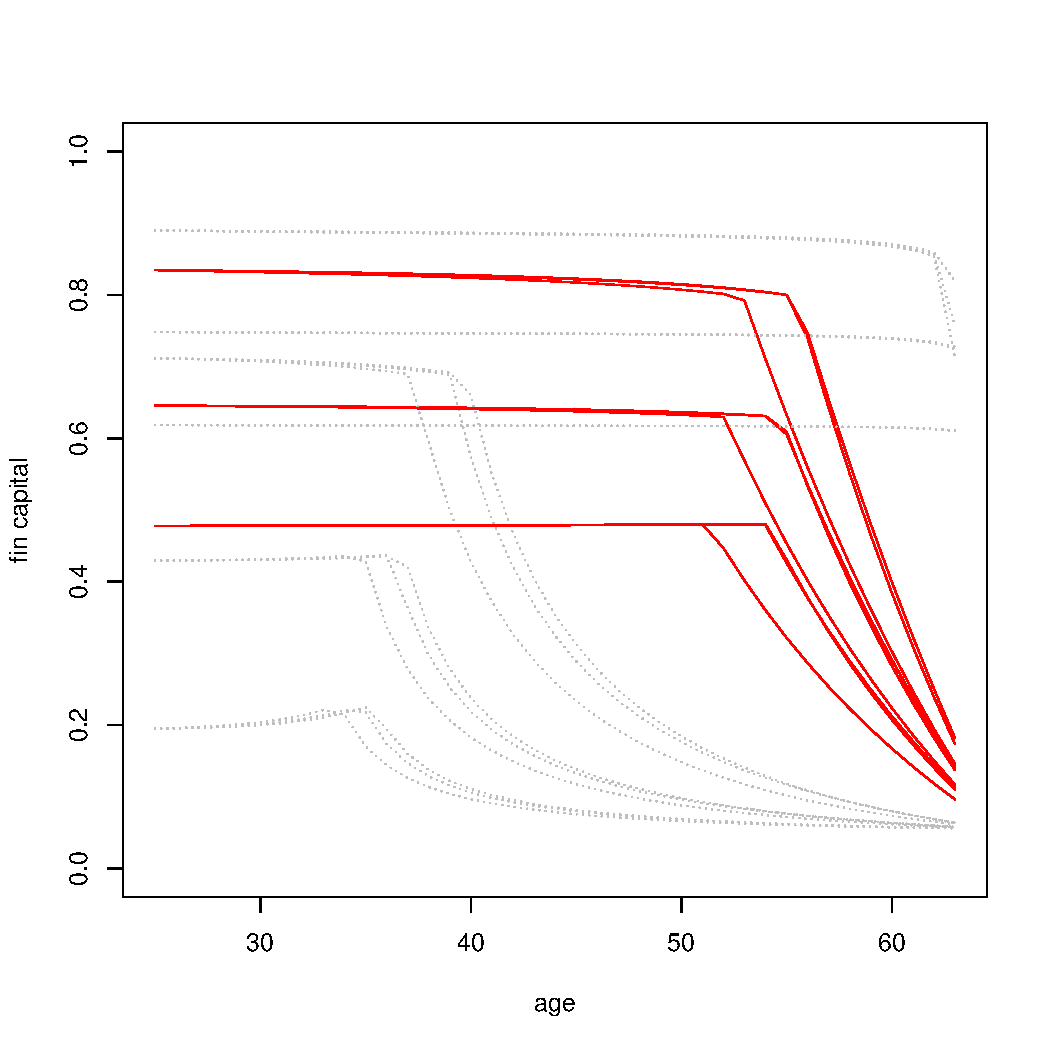
\includegraphics[scale=0.4]{figs/hmunkhouse10.pdf}
		\caption{Housing for $\gamma = 10$}
	\end{subfigure}
	\caption{Munk's stock and housing shares for different wage growth, stock-wage correlation and risk aversion levels}
\end{figure}

\subsection{Early results}

After a lifetime of investing in the above portfolios, the household accumulates different levels of wealth, summarized in Table 5.1. Since the consumption preferences are monotonic, we can make early conclusions even without calculating expected utilities --- the higher the accumulated wealth, the better: 

\begin{itemize}
\item Considering lifecycles, even naively, like $(100-age)\%$, is better than investing a fixed amount throughout lifetime
\item Different stock-wage correlations don't make much difference in the outcome without housing, and make considerable difference in models with housing
\item Stock-wage correlations are negatively correlated with total wealth
\item The risk aversion is negatively correlated with total wealth for models without housing and positively --- for models with housing
\item Default options are better for people with flat wage growth rate and worse for people with moderate or steep wage curves
\end{itemize}

\newgeometry{top=2cm,bottom=2cm}
\begin{table}%TABLE 5.1
	\centering
	\caption{Total Accumulated Wealth by Investment Option}
	\begin{tabular}[c]{lrrrr}
		\hline
		Option&$\gamma=5$ (default) & $\gamma=1.5$ & $\gamma=3$ & $\gamma=10$\\
		\hline
		\multicolumn{5}{c}{Defaults}\\
		Anadolu Hayat (riskless)&537,309 TL&537,309 TL&537,309 TL&537,309 TL\\
		$(100-age)\%$&1,039,812 TL&1,039,812 TL&1,039,812 TL&1,039,812 TL\\
		Cocco et al.&2,147,019 TL&2,147,019 TL&2,147,019 TL&2,147,019 TL\\
		Markowitz&412,501 TL&1,206,147 TL&550,465 TL&325,428 TL\\
		\multicolumn{5}{c}{}\\
		\multicolumn{5}{c}{Individualized (no housing)}\\
		Merton (steep) & 2,938,506 TL&6,078,824 TL&3,986,493 TL&2,023,847 TL\\
		Merton (moderate) & 1,242,367 TL&2,583,202 TL&1,689,263 TL&853,121 TL\\
		Merton (flat) & 379,516 TL&860,653 TL&529,776 TL&255,587 TL\\
		Munk (steep-hi) & 2,613,595 TL&6,021,186 TL&3,783,643 TL&1,443,410 TL\\
		Munk (steep-mod) & 2,614,594 TL&6,022,182 TL&3,784,641 TL&1,444,411 TL\\	
		Munk (steep-lo) & 2,615,592 TL&6,023,178 TL&3,785,638 TL&1,445,411 TL\\
		Munk (moderate-hi) & 1,102,873 TL&2,558,560 TL&1,602,748 TL&603,991 TL\\
		Munk (moderate-mod) & 1,103,290 TL&2,558,976 TL&1,603,164 TL&604,409 TL\\	
		Munk (moderate-lo) & 1,103,707 TL&2,559,391 TL&1,603,580 TL&604,826 TL\\
		Munk (flat-hi) & 336,116 TL&850,375 TL&501,534 TL&182,719 TL\\
		Munk (flat-mod) & 336,212 TL&850,471 TL&501,630 TL&182,816 TL\\	
		Munk (flat-lo) & 336,308 TL&850,568 TL&501,726 TL&182,912 TL\\
		\multicolumn{5}{c}{}\\
		\multicolumn{5}{c}{Individualized (housing)}\\
		Munk (steep-hi) & 2,516,069 TL&1,850,423 TL&2,170,033 TL&3,666,651 TL\\
		Munk (steep-mod) & 2,619,683 TL&1,885,502 TL&2,244,519 TL&4,546,216 TL\\	
		Munk (steep-lo) & 2,713,638 TL&1,919,640 TL&2,314,174 TL&4,050,822 TL\\
		Munk (moderate-hi) & 1,061,251 TL&777,423 TL&913,347 TL&1,501,775 TL\\
		Munk (moderate-mod) & 1,105,444 TL&792,331 TL&945,023 TL&1,881,273 TL\\	
		Munk (moderate-lo) & 1,145,103 TL&806,841 TL&974,647 TL&1,686,710 TL\\
		Munk (flat-hi) & 328,450 TL&256,110 TL&297,080 TL&426,696 TL\\
		Munk (flat-mod) & 340,351 TL&261,520 TL&307,038 TL&540,733 TL\\	
		Munk (flat-lo) & 355,176 TL&265,574 TL&316,592 TL&479,246 TL\\
		\hline
	\end{tabular}
\end{table}
\resetgeometry

\subsection{Annuitization}
To formalize the observations made in the previous section, we will construct annuities and plug them into expected utility functions. As described in detail in Chapter 3, we define annuities by dividing the total wealth before retirement by the discount factor $1 + \sum^{100}_{t=58}\frac{p_t}{1+r_f}$. Using survival probabilities, obtained from TUIK, and risk-free rate of return, described in the previous chapter, we calculate the discount factor as $205.29$. The annuities are obtained by dividing all the values in the Table 5.1 by $205.29$. The resulting values are presented in Table 5.2. 

\newgeometry{top=2cm,bottom=2cm}
\begin{table}%TABLE 5.2
	\centering
	\caption{Annual Pensions by Investment Option}
	\begin{tabular}[c]{lrrrr}
		\hline
		Option&$\gamma=5$ (default) & $\gamma=1.5$ & $\gamma=3$ & $\gamma=10$\\
		\hline
		\multicolumn{5}{c}{Defaults}\\
		Anadolu Hayat (riskless)&2,617 TL&2,617 TL&2,617&2,617 TL\\
		$(100-age)\%$&5,065 TL&5,065 TL&5,065 TL&5,065 TL\\
		Cocco et al.&10,459 TL&10,459 TL&10,459 TL&10,459 TL\\
		Markowitz&2,009 TL&5,875 TL&2,681 TL&1585 TL\\
		\multicolumn{5}{c}{}\\
		\multicolumn{5}{c}{Individualized (no housing)}\\
		Merton (steep) &14,314 TL&29,611 TL&19,419 TL&9,859 TL\\
		Merton (moderate) &6,052 TL&12,583 TL&8,229 TL&4,156 TL\\
		Merton (flat) & 1,849 TL&4,192 TL&2,581 TL&1,245 TL\\
		Munk (steep-hi) &12,731 TL&29,330 TL&18,431 TL&7,031 TL\\
		Munk (steep-mod)&12,736 TL&29,335 TL&18,436 TL&7,036 TL\\
		Munk (steep-lo) &12,741 TL&29,340 TL&18,441 TL&7,041 TL\\
		Munk (moderate-hi)&5,372 TL&12,463 TL&7,807 TL&2,942 TL\\
		Munk (moderate-mod)&5,374 TL&12,465 TL&7,809 TL&2,944 TL\\
		Munk (moderate-lo)&5,376 TL&12,467 TL&7,811 TL&2,946 TL\\
		Munk (flat-hi) &1,637 TL&4,142 TL&2,443 TL&890 TL\\
		Munk (flat-mod) &1,638 TL&4,143 TL&2,444 TL&891 TL\\
		Munk (flat-lo) &1,638 TL&4,143 TL&2,444 TL&891 TL\\
		\multicolumn{5}{c}{}\\
		\multicolumn{5}{c}{Individualized (housing)}\\
		Munk (steep-hi) &12,256 TL&9,014 TL&10,571 TL&17,861 TL\\
		Munk (steep-mod) & 12,761 TL&9,185 TL&10,933 TL&22,146 TL\\
		Munk (steep-lo) &13,219 TL&9,351 TL&11,273 TL&19,732 TL\\
		Munk (moderate-hi)&5,170 TL&3,787 TL&4,449 TL&7,315 TL\\
		Munk (moderate-mod)&5,385 TL&3,860 TL&4,603 TL&9,164 TL\\
		Munk (moderate-lo)&5,578 TL&3,930 TL&4,748 TL&8,216 TL\\
		Munk (flat-hi) & 1,600 TL&1,248 TL&1,447 TL&2,079 TL\\
		Munk (flat-mod) &1,658 TL&1,274 TL&1,496 TL&2,634 TL\\
		Munk (flat-lo) & 1,730 TL&1,294 TL&1,542 TL&2,335 TL\\
		\hline
	\end{tabular}
\end{table}
\resetgeometry


\subsection{Consumption during retirement}
We model that the individuals spend their annuity returns to consume baskets which cost $100$ TL during the year, when our agent is 58 years old, and increase by inflation rate $\pi = 8.4\%$. Thus, every period $t>57$ our agent consumes $\frac{annuity}{100\cdot\left(1.084\right)^{t-58}}$. We do not provide the separate table with the value streams, as they will be implicitly included in utility values.

\subsection{Expected utilities}
Finally, we will plug the consumption streams, calculated in the previous section, into the constant relative risk-aversion expected utility functions to compare the welfare effects. The resulting expected utility values are presented in Table 5.3.

\subsection{Conclusions}
Now, we can observe the final resutls:

\begin{itemize}

\item Naive lifecycle investment portfolios, such as $(100-age)\%$ don't overperform fixed-ratio Markowitz, because they don't take the risk aversion into consideration.
\item Cocco et al.'s $(200-2.5\cdot age)\%$ approximation is the best default portfolio. It is easy to interpret and captures lifecycle effect.
\item All models perform better for higher risk aversion and worse for lower risk aversion.
\item Higher stock-wage correlation considerably decreases the utility for moderate and flat wages, and doesn't affect much for steep wages.
\item Merton's solution outperforms Munk's solution without housing for low levels of risk aversion, and performs save for high level of risk aversion ($\gamma=10$).
\item Munk's solution with housing outperforms every other solution for high levels of risk aversion ($\gamma=10$).
\item Munk's solution with housing outperforms Munk's solution without housing for $\gamma=5,10$.
\item Markowitz's solution outperforms both Merton's and Munk's solutions for flat wages.
\item Individualizing lifecycles by wage growth rate and stock-wage correlation increases welfare for steep wagers and decreases welfare for flat wagers.
\end{itemize}

\paragraph{}We did not provide numerical conclusions, since they are trivial --- they can be obtained by calculating percentage differences in Table 5.3.

\newgeometry{top=2cm,bottom=2cm}
\begin{table}%TABLE 5.3
	\centering
	\caption{Expected Utilities by Investment Option}
	\begin{tabular}[c]{lrrrr}
		\hline
		Option&$\gamma=5$ (default) & $\gamma=1.5$ & $\gamma=3$ & $\gamma=10$\\
		\hline
\multicolumn{5}{c}{Defaults}\\
Anadolu Hayat (riskless)&-0.0014323&-3.8493850&-0.0323960&-0.0001696\\
$(100-age)\%$&-0.0001021&-2.7671080&-0.0086503&-0.0000004\\
Cocco et al.&-0.0000056&-1.9256860&-0.0020289&0.0000000\\
Markowitz&-0.0000564&-2.5692320&-0.0064289&-0.0000001\\
\multicolumn{5}{c}{}\\
\multicolumn{5}{c}{Individualized (no housing)}\\
Merton (steep) &-0.0000016&-1.1444420&-0.0005885&0.0000000\\
Merton (moderate) &-0.0000501&-1.7555950&-0.0032775&-0.0000026\\
Merton (flat) &-0.0057545&-3.0415100&-0.0333239&-0.1360504\\
Munk (steep-hi) &-0.0000026&-1.1499060&-0.0006533&0.0000000\\
Munk (steep-mod)&-0.0000026&-1.1498110&-0.0006530&0.0000000\\
Munk (steep-lo) &-0.0000026&-1.1497160&-0.0006526&0.0000000\\
Munk (moderate-hi)&-0.0000807&-1.7640290&-0.0036409&-0.0000592\\
Munk (moderate-mod)&-0.0000806&-1.7638860&-0.0036390&-0.0000588\\
Munk (moderate-lo)&-0.0000804&-1.7637420&-0.0036371&-0.0000585\\
Munk (flat-hi) &-0.0093535&-3.0598360&-0.0371825&-2.7892210\\
Munk (flat-mod) &-0.0093428&-3.0596630&-0.0371682&-2.7759950\\
Munk (flat-lo) &-0.0093321&-3.0594900&-0.0371540&-2.7628600\\
\multicolumn{5}{c}{}\\
\multicolumn{5}{c}{Individualized (housing)}\\
Munk (steep-hi) &-0.0000030&-2.0742830&-0.0019861&0.0000000\\
Munk (steep-mod) &-0.0000025&-2.0548970&-0.0018565&0.0000000\\
Munk (steep-lo) &-0.0000022&-2.0365430&-0.0017464&0.0000000\\
Munk (moderate-hi)&-0.0000941&-3.2001820&-0.0112116&0.0000000\\
Munk (moderate-mod)&-0.0000799&-3.1699320&-0.0104726&0.0000000\\
Munk (moderate-lo)&-0.0000694&-3.1412990&-0.0098457&0.0000000\\
Munk (flat-hi) &-0.0102577&-5.5755810&-0.1059719&-0.0013504\\
Munk (flat-mod) &-0.0088965&-5.5176110&-0.0992097&-0.0001602\\
Munk (flat-lo) &-0.0075016&-5.4753340&-0.0933124&-0.0004748\\
		\hline
	\end{tabular}
\end{table}
\resetgeometry

